% !TEX program = xelatex
% Компилировать XeLaTeX (или LuaLaTeX). pdfLaTeX тоже поддержан (ветка с T2A).
\documentclass[11pt,a4paper]{article}

\usepackage{iftex}
\usepackage{amsmath,amssymb}
\ifPDFTeX
  \usepackage{cmap}
  \usepackage[T2A]{fontenc}
  \usepackage[utf8]{inputenc}
  \usepackage[english,russian]{babel}
  \newcommand{\spaced}[1]{#1}
\else
  \usepackage[english]{babel}
  \babelprovide[import,main]{russian}
  \usepackage{fontspec}
  \IfFontExistsTF{Liberation Serif}{\setmainfont{Liberation Serif}}{%
    \IfFontExistsTF{Times New Roman}{\setmainfont{Times New Roman}}{%
      \setmainfont{cmunrm.otf}[BoldFont=cmunbx.otf,ItalicFont=cmunti.otf,BoldItalicFont=cmunbi.otf]}}
  \IfFontExistsTF{Liberation Sans}{\setsansfont{Liberation Sans}}{%
    \IfFontExistsTF{Arial}{\setsansfont{Arial}}{%
      \setsansfont{cmunss.otf}[BoldFont=cmunsx.otf,ItalicFont=cmunsi.otf,BoldItalicFont=cmunso.otf]}}
  \newcommand{\spaced}[1]{{\addfontfeatures{LetterSpace=8}#1}}
\fi

\usepackage[left=2cm,right=1.5cm,top=1.8cm,bottom=2cm]{geometry}
\usepackage{icomma}
\usepackage{graphicx}
\usepackage{array,longtable,multirow,makecell}
\usepackage{enumitem}
\usepackage{xcolor}
\usepackage{tikz}
\usetikzlibrary{arrows.meta}
\usepackage{pgfplots}
\pgfplotsset{compat=1.17}

\setlist[itemize]{label=\textbullet, leftmargin=1.6em, itemsep=2pt, topsep=4pt}
\setlength{\parindent}{0pt}
\setlength{\parskip}{3pt}
\renewcommand{\arraystretch}{1.25}

% заголовок раздела в стиле бланка
\newcommand{\sect}[1]{\par\vspace{10pt}{\large #1}\par\vspace{4pt}}
% ячейка с формулой в таблице рабочих формул
\newcommand{\F}[1]{\begin{minipage}[c]{\linewidth}\centering\vspace*{5pt}$\displaystyle #1$\par\vspace{5pt}\end{minipage}}
\newcommand{\D}[1]{\begin{minipage}[c]{\linewidth}\raggedright\vspace*{3pt}#1\par\vspace{3pt}\end{minipage}}
\newcommand{\gr}{\ensuremath{^\circ}}
\newcommand{\sub}[1]{\text{#1}}

% стиль «миллиметровки» для графиков
\pgfplotsset{
  mmpaper/.style={
    width=16cm, height=12cm,
    axis lines=left,
    axis line style={-{Stealth[length=3mm]}, thick},
    grid=both,
    minor tick num=4,
    major grid style={cyan!70!blue!45, line width=0.45pt},
    minor grid style={cyan!45!white!60, line width=0.2pt},
    tick style={black, thick},
    tick align=center,
    /pgf/number format/.cd, use comma, 1000 sep={},
  },
}

\begin{document}

% ---------------------------------------------------------------- шапка
\begin{minipage}[c]{0.55\textwidth}
  \centering\small\bfseries
  Университет ИТМО\\
  Физико-технический мегафакультет\\
  Физический факультет
\end{minipage}\hfill
\begin{minipage}[c]{0.4\textwidth}
  \centering
  \IfFileExists{itmo_logo.png}{\includegraphics[height=1.3cm]{itmo_logo.png}}{{\sffamily\bfseries\fontsize{34}{36}\selectfont ITMO}}
\end{minipage}

\vspace{4pt}\hrule\vspace{6pt}

{\small
\begin{tabular}{@{}p{0.52\textwidth}@{}p{0.46\textwidth}@{}}
Группа \underline{\makebox[5.6cm][l]{ФИЗ ПИИКТ 2.1.1}} & К работе допущен\underline{\makebox[4.2cm]{}}\\
Студент \underline{\makebox[5.5cm][l]{Бригада 8 (Добкес, Пегушина)}} & Работа выполнена\underline{\makebox[4.1cm]{}}\\
Преподаватель \underline{\makebox[4.4cm][l]{Сорокина Елена}} & Отчет принят\underline{\makebox[4.75cm]{}}\\
\underline{\makebox[3.2cm][l]{Константиновна}} & \\
\end{tabular}}

\vspace{8pt}
\begin{center}
  {\LARGE\bfseries \spaced{Рабочий протокол и отчет по}\\[2pt]
   \spaced{лабораторной работе № 1.05}}\\[8pt]
  {\Large Исследование колебаний физического маятника}
\end{center}
\vspace{2pt}\hrule

% ---------------------------------------------------------------- 1
\sect{1. Цель работы.}
\begin{itemize}
  \item Изучение характеристик затухающих колебаний физического маятника.
\end{itemize}

% ---------------------------------------------------------------- 2
\sect{2. Задачи, решаемые при выполнении работы.}
\begin{itemize}
  \item Измерить период затухающих колебаний.
  \item Определить вид зависимости амплитуды затухающих колебаний физического маятника от времени.
  \item Определить вид зависимости периода колебаний от момента инерции физического маятника.
  \item Определить преобладающий тип трения.
  \item Определить экспериментальную и теоретическую приведённые длины маятника при его разных конфигурациях.
\end{itemize}

% ---------------------------------------------------------------- 3
\sect{3. Объект исследования.}
Физический маятник — передняя крестовина, состоящая из ступицы с четырьмя спицами, на каждой из которых
закреплён груз на регулируемом расстоянии от оси. Крестовина совершает колебания вокруг неподвижной
горизонтальной оси, проходящей через ступицу. 

% ---------------------------------------------------------------- 4
\sect{4. Метод экспериментального исследования.}
Метод основан на измерении секундомером времени свободных затухающих колебаний маятника: моментов времени,
в которые амплитуда уменьшается от $\varphi_0=30\gr$ до $25\gr$, $20\gr$, $15\gr$, $10\gr$, $5\gr$, и времени десяти
колебаний при различных положениях боковых грузов. По виду зависимости $\varphi=f(t)$, аппроксимированной
методом наименьших квадратов, определяется преобладающий тип трения и полуширина зоны застоя $\varphi_\sub{з}$;
по зависимости $T^2=f(I)$ — произведение $m\ell$; по периодам колебаний — приведённая длина маятника $\ell_\sub{пр}$.

% ---------------------------------------------------------------- 5
\sect{5. Рабочие формулы и исходные данные.}
Рабочие формулы:

\begin{longtable}{|>{\centering\arraybackslash}m{0.9cm}|m{7.6cm}|m{7.3cm}|}
\hline
1 & \F{\langle t\rangle=\frac{1}{n}\sum_{i=1}^{n}t_i} & \D{Среднее арифметическое выборки}\\\hline
2 & \F{S_{\langle t\rangle}=\sqrt{\frac{\sum\limits_{i=1}^{n}\left(t_i-\langle t\rangle\right)^2}{n(n-1)}}} & \D{Среднее квадратичное отклонение среднего}\\\hline
3 & \F{\Delta_{\langle t\rangle}=t_{\alpha,n}\,S_{\langle t\rangle}} & \D{Случайная погрешность ($t_{0,95;\,3}=4,30$)}\\\hline
4 & \F{\Delta_t=\sqrt{\Delta_{\langle t\rangle}^2+\left(\frac{2}{3}\,\Delta_\sub{и}\right)^2}} & \D{Абсолютная погрешность измерения времени}\\\hline
5 & \F{\delta_t=\frac{\Delta_t}{\langle t\rangle}\cdot100\,\%} & \D{Относительная погрешность измерения времени}\\\hline
6 & \F{T=\frac{\langle t\rangle}{N},\qquad \Delta_T=\frac{\Delta_t}{N}} & \D{Период колебаний и его абсолютная погрешность}\\\hline
7 & \F{\varphi_m=\varphi_0e^{-\beta t}\;\Rightarrow\;\ln\frac{\varphi_m}{\varphi_0}=-\beta t} & \D{Затухание амплитуды при вязком трении}\\\hline
8 & \F{\varphi(t)=\varphi_0-\frac{4\varphi_\sub{з}}{T}\,t} & \D{Затухание амплитуды при сухом трении ($\varphi(nT)=\varphi_0-4n\varphi_\sub{з}$)}\\\hline
9 & \F{\varphi_\sub{з}=\frac{k\,T}{4}} & \D{Полуширина зоны застоя ($k=|b|$ — модуль углового коэффициента прямой $\varphi=f(t)$)}\\\hline
10 & \F{n_\sub{ост}=\left[\frac{|\varphi_0|-\varphi_\sub{з}}{2\varphi_\sub{з}}\right],\qquad t_\sub{ост}=n_\sub{ост}\cdot\frac{T}{2}} & \D{Число полупериодов и время до остановки маятника}\\\hline
11 & \F{R=\ell_1+(n-1)\,\ell_0+\frac{h_\sub{гр}}{2}} & \D{Расстояние от оси вращения до центра груза на $n$-й риске}\\\hline
12 & \F{I_\sub{гр}=m_\sub{гр}\left(R_\sub{в}^2+R_\sub{н}^2+2R_\sub{б}^2\right)} & \D{Момент инерции грузов относительно оси вращения}\\\hline
13 & \F{I=I_\sub{гр}+I_0} & \D{Полный момент инерции маятника}\\\hline
14 & \F{T=2\pi\sqrt{\frac{I}{mg\ell}}\;\Rightarrow\;T^2=\frac{4\pi^2}{mg\ell}\,I} & \D{Период физического маятника; линейная зависимость $T^2=f(I)$}\\\hline
15 & \F{m\ell=\frac{4\pi^2}{b\,g}} & \D{Произведение $m\ell$ по угловому коэффициенту $b$ прямой $T^2=f(I)$}\\\hline
16 & \F{m\ell_\sub{теор}=m_\sub{гр}\left(R_\sub{н}-R_\sub{в}\right)} & \D{Теоретическое значение $m\ell$}\\\hline
17 & \F{\ell_\sub{пр эксп}=\frac{gT^2}{4\pi^2}} & \D{Экспериментальная приведённая длина}\\\hline
18 & \F{\ell_\sub{пр теор}=\frac{I}{m\ell_\sub{теор}}} & \D{Теоретическая приведённая длина}\\\hline
19 & \F{\Delta_\sub{откл}=\left|\ell_\sub{пр эксп}-\ell_\sub{пр теор}\right|\newline \delta_\sub{откл}=\frac{\Delta_\sub{откл}}{\ell_\sub{пр теор}}\cdot100\,\%} & \D{Абсолютное и относительное отклонение $\ell_\sub{пр эксп}$ от $\ell_\sub{пр теор}$}\\\hline
\multicolumn{3}{|c|}{\rule{0pt}{14pt}Метод наименьших квадратов для зависимостей $y=a+bx$, где $y=\varphi,\ T^2$;\ $x=t,\ I$;\ $n=6$}\\\hline
20 & \F{\bar x=\frac{1}{n}\sum_{i=1}^{n}x_i,\qquad \bar y=\frac{1}{n}\sum_{i=1}^{n}y_i} & \D{Средние значения}\\\hline
21 & \F{b=\frac{\sum\limits_{i=1}^{n}\left(x_i-\bar x\right)\left(y_i-\bar y\right)}{\sum\limits_{i=1}^{n}\left(x_i-\bar x\right)^2}} & \D{Угловой коэффициент}\\\hline
22 & \F{a=\bar y-b\,\bar x} & \D{Свободный член}\\\hline
23 & \F{d_i=y_i-\left(a+bx_i\right)} & \D{Отклонение точки от прямой}\\\hline
24 & \F{D=\sum_{i=1}^{n}\left(x_i-\bar x\right)^2} & \D{Вспомогательная величина}\\\hline
25 & \F{S_b^2=\frac{1}{D}\,\frac{\sum d_i^2}{n-2}} & \D{Дисперсия углового коэффициента}\\\hline
26 & \F{S_a^2=\left(\frac{1}{n}+\frac{\bar x^{\,2}}{D}\right)\frac{\sum d_i^2}{n-2}} & \D{Дисперсия свободного члена}\\\hline
27 & \F{\Delta_b=2S_b,\qquad \Delta_a=2S_a} & \D{Абсолютные погрешности коэффициентов ($P\approx0,95$)}\\\hline
28 & \F{\delta_{\varphi_\sub{з}}=\sqrt{\left(\frac{\Delta_k}{k}\right)^2+\left(\frac{\Delta_T}{T}\right)^2}} & \D{Относительная погрешность $\varphi_\sub{з}$ ($\Delta_k=\Delta_b$)}\\\hline
29 & \F{\Delta_{m\ell}=m\ell\cdot\frac{\Delta_b}{b}} & \D{Абсолютная погрешность $m\ell$ ($g$ — константа)}\\\hline
30 & \F{\Delta\ell_\sub{пр эксп}=\ell_\sub{пр эксп}\cdot\frac{2\Delta_T}{T}} & \D{Абсолютная погрешность $\ell_\sub{пр эксп}$}\\\hline
31 & \F{\Delta_R=\sqrt{\Delta_{\ell_1}^2+\left((n-1)\Delta_{\ell_0}\right)^2+\left(\frac{\Delta_{h_\sub{гр}}}{2}\right)^2}} & \D{Абсолютная погрешность расстояния $R$}\\\hline
32 & \F{\delta_{m\ell_\sub{теор}}=\sqrt{\left(\frac{\Delta_{m_\sub{гр}}}{m_\sub{гр}}\right)^2+\frac{\Delta_{R_\sub{н}}^2+\Delta_{R_\sub{в}}^2}{\left(R_\sub{н}-R_\sub{в}\right)^2}}} & \D{Относительная погрешность $m\ell_\sub{теор}$}\\\hline
\end{longtable}

Исходные данные:

На рисунке 1 приведена схема экспериментального стенда. В ступице Ст закреплены четыре спицы Сп, на каждой из которых размещён груз Гр. Расстояние от центра масс системы из ступицы, грузов и спиц до оси вращения крестовины — $\ell$. Расстояния $R_\sub{в}$, $R_\sub{н}$ и $R_\sub{б}$ — это расстояния от центров масс верхнего, нижнего и боковых грузов до оси вращения крестовины. Эти расстояния можно регулировать, изменяя тем самым момент инерции крестовины с грузами. Ось качания (ось подвеса) проходит перпендикулярно рисунку через точку $O$. Точка $C$ — центр масс маятника. Угол $\varphi$ между вертикалью и прямой $OC$, проведённой из точки подвеса к центру масс перпендикулярно оси вращения, задаёт текущее положение маятника. $g$ — ускорение свободного падения.


На рисунке 2 приведена упрощённая схема одной спицы со ступицей, где $\ell_1$ — расстояние от оси вращения до первой риски, $\ell_0$ — расстояние между соседними рисками, $b=h_\sub{гр}$ — размер груза вдоль спицы, $m_\sub{гр}$ и $d_\sub{гр}$ — масса и диаметр груза на крестовине.

\begin{center}
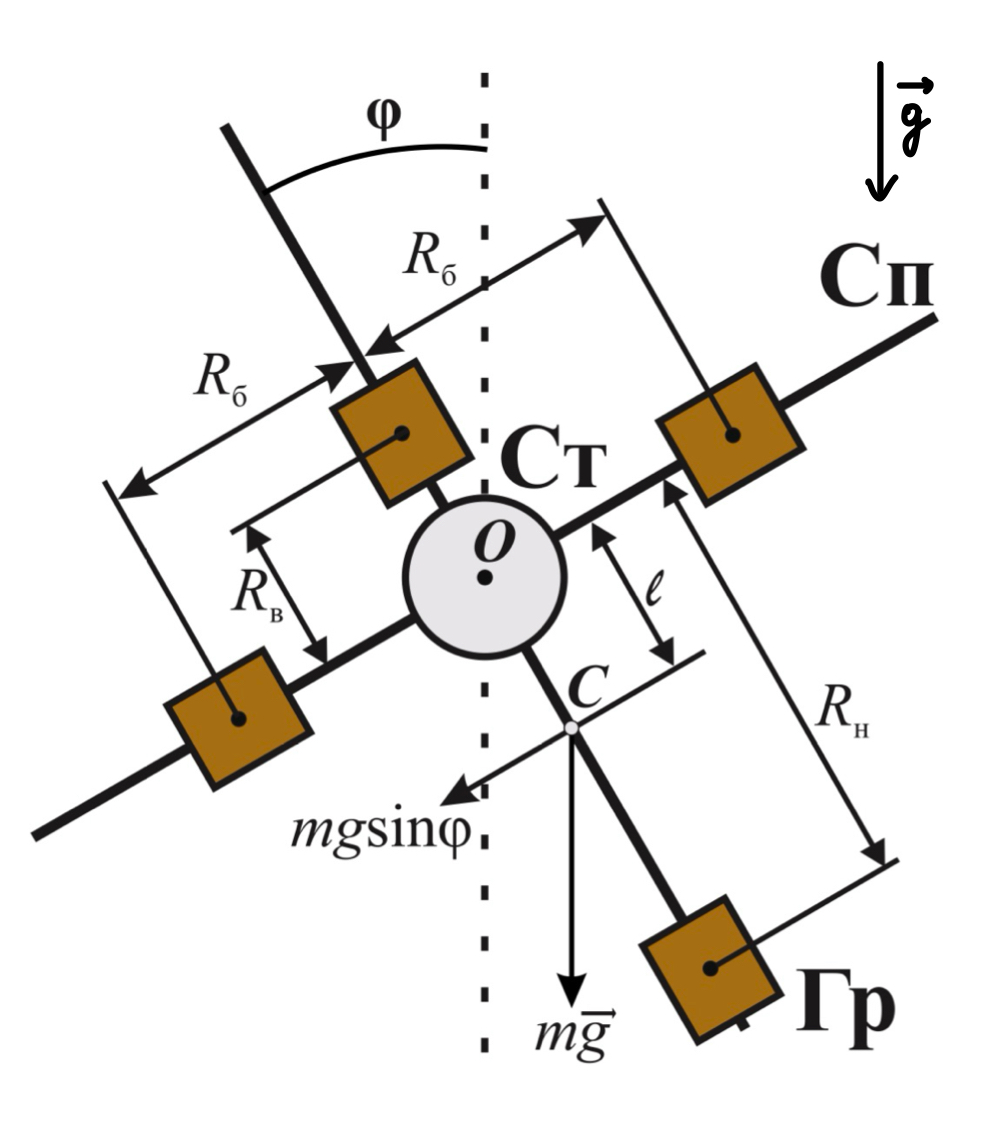
\includegraphics[width=0.6\textwidth]{scheme2.jpeg}\newline
    \small Рисунок 1
\end{center}

\begin{center}
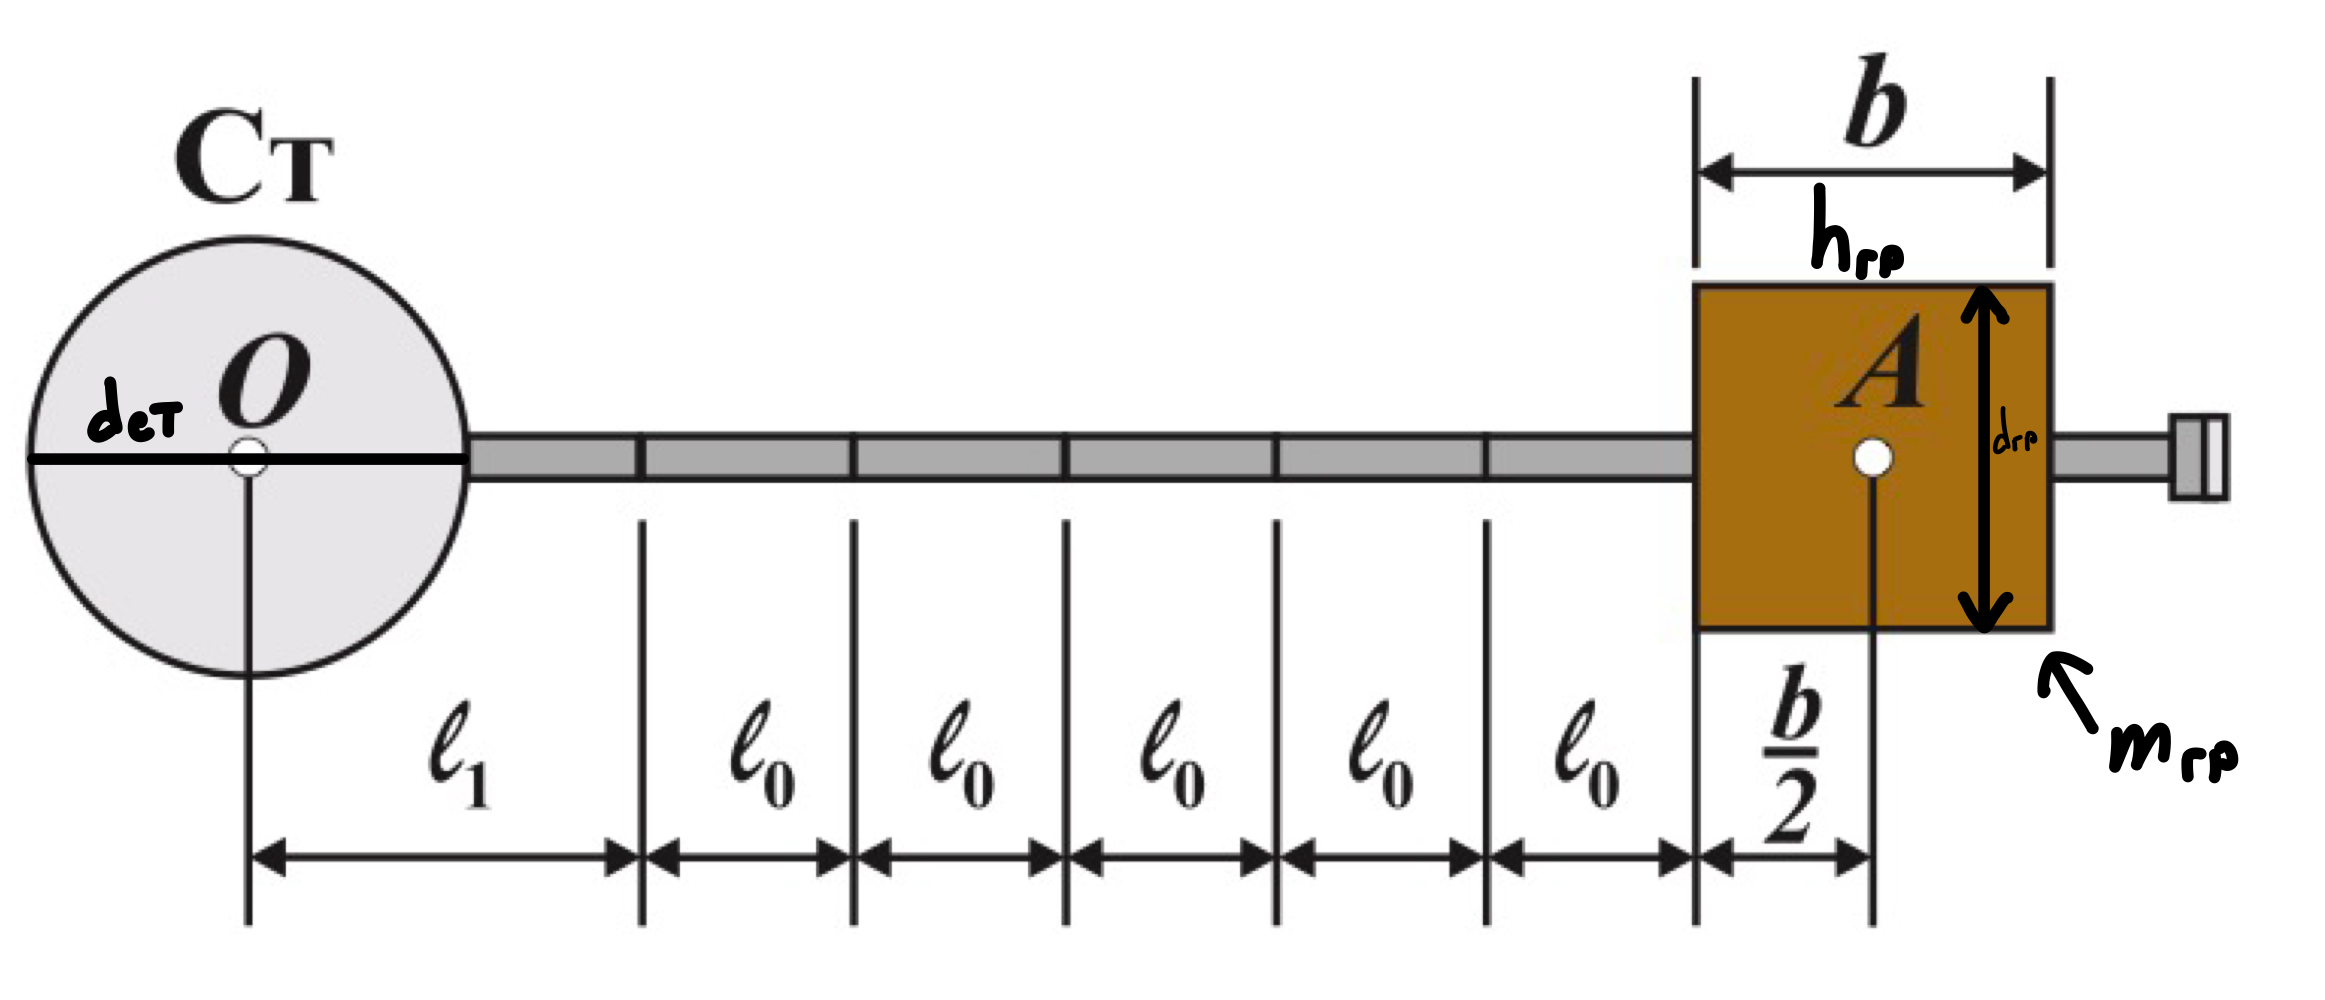
\includegraphics[width=0.8\textwidth]{scheme_part.jpeg}\newline
    \small Рисунок 2
\end{center}

% ---------------------------------------------------------------- 6
\sect{6-8. Измерительные приборы. Результаты прямых измерений и их обработки}
\clearpage

% ---------------------------------------------------------------- 9
\sect{9. Расчет результатов косвенных измерений (таблицы, примеры расчетов).}

\begin{center}
Таблица 1 – Расчетные величины среднего времени и периода колебаний при амплитуде $\varphi=30\gr$\\[3pt]
\begin{tabular}{|c|c|c|c|c|c|}
\hline
\makecell{Количество\\колебаний $N$} & $\langle t\rangle$, с & $\Delta_t$, с & $\delta_t$, \% & $T$, с & $\Delta_T$, с\\\hline
10 & 18,53 & 1,1 & 6,0 & 1,853 & 0,11\\\hline
\end{tabular}
\end{center}

Приведем пример расчета для таблицы 1.

По формуле (1) найдем среднее время десяти колебаний:
\[
\langle t\rangle=\frac{18,82+18,02+18,76}{3}=18,53\ \text{с}.
\]
По формуле (6) найдем период колебаний:
\[
T=\frac{18,53}{10}=1,853\ \text{с}.
\]

\begin{center}
Таблица 2 – Расчетные величины среднего времени колебаний при различной амплитуде колебаний\\[3pt]
\begin{tabular}{|c|c|}
\hline
\makecell{Амплитуда\\отклонения $\varphi_i$, $^\circ$} & \makecell{Среднее время\\колебаний $\langle t\rangle$, с}\\\hline
25 & 39,82\\\hline
20 & 81,78\\\hline
15 & 130,57\\\hline
10 & 191,36\\\hline
5 & 261,12\\\hline
\end{tabular}
\end{center}

Приведем пример расчета первой строки таблицы 2 ($\varphi=25\gr$).
По формуле (1):
\[
\langle t\rangle=\frac{37,86+38,86+42,73}{3}=39,82\ \text{с}.
\]

Можно заметить, что за каждый период график зависимости амплитуды колебаний от времени $\varphi=f(t)$ уменьшается на одну и ту же величину $4\varphi_\sub{з}$ и экспериментальные точки в пределах погрешностей ложатся на прямую, следовательно, в затухании колебаний преобладает сухое трение (трение в оси подвеса).
\newline
\newline
Используя метод МНК (формулы 20–22), найдем коэффициенты линейной зависимости $\varphi=a+bt$ амплитуды колебаний $\varphi$ от времени $t$, $b$ — скорость убывания амплитуды, $a$ — начальная амплитуда по прямой:
\[
\bar t=\frac{0+39,82+81,78+130,57+191,36+261,12}{6}=117,44\ \text{с},\qquad
\bar\varphi=\frac{30+25+20+15+10+5}{6}=17,50\gr,
\]
\[
b=\frac{\sum\limits_{i=1}^{6}(t_i-117,44)(\varphi_i-17,50)}{\sum\limits_{i=1}^{6}(t_i-117,44)^2}
=\frac{-4522,5}{47368,6}=-0,0955\ {}^\circ/\text{с},
\]
\[
a=17,50-(-0,0955)\cdot117,44=28,71\gr.
\]
Таким образом, $\varphi(t)=28,71-0,0955\,t$ ($\varphi$ — в градусах, $t$ — в секундах): амплитуда убывает со скоростью
$0,0955\ {}^\circ/\text{с}$, начальная амплитуда по прямой $28,71\gr$.
Модуль углового коэффициента $k=|b|=0,0955\ {}^\circ/\text{с}$. По формуле (9) найдем полуширину зоны застоя:
\[
\varphi_\sub{з}=\frac{0,0955\cdot1,853}{4}=0,0442\gr=7,72\cdot10^{-4}\ \text{рад}.
\]
По формуле (10) оценим, через сколько колебаний маятник остановится:
\[
n_\sub{ост}=\left[\frac{30-0,0442}{2\cdot0,0442}\right]=[338,6]=338\ \text{полупериодов}\ (\approx169\ \text{периодов})
\]

\begin{center}
Таблица 3 – Расчетные величины среднего времени и периода колебаний при различных положениях боковых грузов\\[3pt]
\begin{tabular}{|c|c|c|c|c|c|c|}
\hline
\makecell{Положение\\боковых грузов} & \makecell{Среднее время\\колебаний $\langle t\rangle$, с} & $\Delta_t$, с & $\delta_t$, \% & \makecell{Период\\колебаний $T$, с} & $\Delta_T$, с & $\delta_T$, \%\\\hline
1 риска & 16,38 & 0,49 & 3,0 & 1,638 & 0,049 & 3,0\\\hline
2 риска & 17,48 & 0,43 & 2,5 & 1,748 & 0,043 & 2,5\\\hline
3 риска & 18,63 & 0,57 & 3,1 & 1,863 & 0,057 & 3,1\\\hline
4 риска & 19,76 & 0,27 & 1,4 & 1,976 & 0,027 & 1,4\\\hline
5 риска & 21,27 & 1,1 & 5,0 & 2,127 & 0,11 & 5,0\\\hline
6 риска & 22,78 & 0,68 & 3,0 & 2,278 & 0,068 & 3,0\\\hline
\end{tabular}
\end{center}

Приведем пример расчета первой строки таблицы 3 (боковые грузы на 1 риске).
По формулам (1) и (6):
\[
\langle t\rangle=\frac{16,20+16,59+16,34}{3}=16,38\ \text{с},\qquad T=\frac{16,38}{10}=1,638\ \text{с}.
\]

\begin{center}
Таблица 4 – Расчетные величины\\[3pt]
\small
\begin{tabular}{|l|c|c|c|c|c|c|}
\hline
\multirow{2}{*}{Расчетная величина} & \multicolumn{6}{c|}{Номер риски}\\\cline{2-7}
 & 1 & 2 & 3 & 4 & 5 & 6\\\hline
$R_\sub{в}$, мм & 77,0 & 77,0 & 77,0 & 77,0 & 77,0 & 77,0\\\hline
$R_\sub{н}$, мм & 202,0 & 202,0 & 202,0 & 202,0 & 202,0 & 202,0\\\hline
$R_\sub{б}$, мм & 77,0 & 102,0 & 127,0 & 152,0 & 177,0 & 202,0\\\hline
$I_\sub{гр}$, кг$\cdot$м$^2$ & 0,02391 & 0,02756 & 0,03223 & 0,03792 & 0,04463 & 0,05236\\\hline
$I$, кг$\cdot$м$^2$ & 0,03191 & 0,03556 & 0,04023 & 0,04592 & 0,05263 & 0,06036\\\hline
$T^2$, с$^2$ & 2,682 & 3,056 & 3,470 & 3,905 & 4,526 & 5,189\\\hline
$\ell_\sub{пр эксп}$, мм & 667,1 & 760,0 & 863,0 & 971,2 & 1125,7 & 1290,8\\\hline
$\Delta\ell_\sub{пр эксп}$, мм & 40 & 37 & 53 & 27 & 113 & 77\\\hline
$\ell_\sub{пр теор}$, мм & 625,6 & 697,2 & 788,8 & 900,4 & 1032,0 & 1183,6\\\hline
$\Delta_\sub{откл}$, мм & 41,5 & 62,8 & 74,2 & 70,8 & 93,7 & 107,2\\\hline
$\delta_\sub{откл}$, \% & 6,6 & 9,0 & 9,4 & 7,9 & 9,1 & 9,1\\\hline
\end{tabular}
\end{center}

Приведем пример расчета первого столбца таблицы 4 (боковые грузы на 1 риске).

По формуле (11) найдем расстояния от оси вращения до центров грузов (верхний — 1 риска, нижний — 6 риска):
\[
R_\sub{в}=57,0+0\cdot25,0+\frac{40,0}{2}=77,0\ \text{мм},\qquad
R_\sub{н}=57,0+5\cdot25,0+\frac{40,0}{2}=202,0\ \text{мм},\qquad
R_\sub{б}=77,0\ \text{мм}.
\]
По формуле (12) найдем момент инерции грузов:
\[
I_\sub{гр}=0,408\cdot\left(0,077^2+0,202^2+2\cdot0,077^2\right)=0,408\cdot0,058591=0,023905\ \text{кг}\cdot\text{м}^2.
\]
По формуле (13) найдем полный момент инерции:
\[
I=0,023905+0,008=0,031905\ \text{кг}\cdot\text{м}^2.
\]

Используя метод МНК (формулы 20–22), найдем коэффициенты линейной зависимости $T^2=a+bI$ квадрата периода колебаний $T^2$ от момента инерции маятника $I$, $b=4\pi^2/(mg\ell)$ — угловой коэффициент, $a$ — свободный член:
\[
\bar I=\frac{0,03191+0,03556+0,04023+0,04592+0,05263+0,06036}{6}=0,044\ \text{кг}\cdot\text{м}^2,
\]
\[
\overline{T^2}=\frac{2,682+3,056+3,470+3,905+4,526+5,189}{6}=3,80\ \text{с}^2,
\]
\[
b=\frac{\sum\limits_{i=1}^{6}(I_i-0,04443)(T_i^2-3,804)}{\sum\limits_{i=1}^{6}(I_i-0,04443)^2}
=\frac{0,05024}{0,0005766}=87,13\ \frac{\text{с}^2}{\text{кг}\cdot\text{м}^2},
\]
\[
a=3,804-87,13\cdot0,04443=-0,067\ \text{с}^2.
\]
Таким образом, $T^2=-0,067+87,13\,I$ ($T^2$ — в с$^2$, $I$ — в кг$\cdot$м$^2$): угловой коэффициент
$4\pi^2/(mg\ell)=87,13\ \text{с}^2/(\text{кг}\cdot\text{м}^2)$, свободный член $-0,067$ с$^2$.
По формуле (15) найдем произведение $m\ell$:
\[
m\ell=\frac{4\pi^2}{87,13\cdot9,82}=\frac{39,48}{855,6}=0,0461\ \text{кг}\cdot\text{м}.
\]
По формуле (16) найдем теоретическое значение $m\ell$:
\[
m\ell_\sub{теор}=0,408\cdot(0,202-0,077)=0,0510\ \text{кг}\cdot\text{м}.
\]
По формуле (17) найдем экспериментальную приведённую длину:
\[
\ell_\sub{пр эксп}=\frac{9,82\cdot1,638^2}{4\pi^2}=\frac{9,82\cdot2,682}{39,48}=0,6671\ \text{м}=667,1\ \text{мм}.
\]
По формуле (18) найдем теоретическую приведённую длину:
\[
\ell_\sub{пр теор}=\frac{0,031905}{0,0510}=0,6256\ \text{м}=625,6\ \text{мм}.
\]
По формуле (19) найдем отклонение:
\[
\Delta_\sub{откл}=|667,1-625,6|=41,5\ \text{мм},\qquad
\delta_\sub{откл}=\frac{41,5}{625,6}\cdot100\,\%=6,6\,\%.
\]

% ---------------------------------------------------------------- 10
\sect{10. Расчет погрешностей измерений (для прямых и косвенных измерений).}

Рассчитаем для значения $\langle t\rangle$ из таблицы 1 абсолютную и относительную погрешности.

По формуле (2) вычислим оценку СКО:
\[
S_{\langle t\rangle}=\sqrt{\frac{(18,82-18,53)^2+(18,02-18,53)^2+(18,76-18,53)^2}{3\cdot2}}=0,2573\ \text{с}.
\]
Рассчитаем величину случайной погрешности по формуле (3), коэффициент Стьюдента $t_{0,95;\,3}=4,30$:
\[
\Delta_{\langle t\rangle}=4,30\cdot0,2573=1,106\ \text{с}.
\]
Вычислим абсолютную погрешность измерения по формуле (4) с учетом случайной и инструментальной погрешности ($\Delta_\sub{и}=0,01$ с):
\[
\Delta_t=\sqrt{1,106^2+\left(\frac{2}{3}\cdot0,01\right)^2}=1,106\ \text{с}.
\]
Определим относительную погрешность по формуле (5) и погрешность периода по формуле (6):
\[
\delta_t=\frac{1,106}{18,53}\cdot100\,\%=6,0\,\%,\qquad \Delta_T=\frac{1,106}{10}=0,11\ \text{с}.
\]
Аналогично для первой строки таблицы 2 ($\varphi=25\gr$): \newline 
$S_{\langle t\rangle}=1,49$ с, $\Delta_t=4,30\cdot1,49=6,4$ с,
$\delta_t=16\,\%$ \newline 
Для первой строки таблицы 3: \newline
$S_{\langle t\rangle}=0,114$ с, $\Delta_t=4,30\cdot0,114=0,49$ с,
$\delta_t=3,0\,\%$, $\Delta_T=0,049$ с.

Используя формулы (23)–(27), найдем погрешности коэффициентов прямой $\varphi=a+bt$:
\begin{align*}
d_1&=30-(28,713-0,09547\cdot0)=1,287\gr\\
d_2&=25-(28,713-0,09547\cdot39,82)=0,089\gr\\
d_3&=20-(28,713-0,09547\cdot81,78)=-0,905\gr\\
d_4&=15-(28,713-0,09547\cdot130,57)=-1,246\gr\\
d_5&=10-(28,713-0,09547\cdot191,36)=-0,443\gr\\
d_6&=5-(28,713-0,09547\cdot261,12)=1,217\gr
\end{align*}
\[
\sum_{i=1}^{6}d_i^2=5,716\ \text{град}^2,\qquad D=47368,6\ \text{с}^2,
\]
\[
S_b^2=\frac{1}{47368,6}\cdot\frac{5,716}{6-2}=3,017\cdot10^{-5}\ \left(^\circ/\text{с}\right)^2,\qquad S_b=0,00549\ {}^\circ/\text{с},
\]
\[
S_a^2=\left(\frac{1}{6}+\frac{117,44^2}{47368,6}\right)\cdot\frac{5,716}{6-2}=0,654\ \text{град}^2,\qquad S_a=0,809\gr,
\]
\[
\Delta_b=2\cdot0,00549=0,011\ {}^\circ/\text{с},\qquad \delta_k=\frac{0,011}{0,0955}\cdot100\,\%=11,5\,\%,\qquad \Delta_a=2\cdot0,809=1,6\gr.
\]
Таким образом, скорость убывания амплитуды $k=(0,095\pm0,011)\ {}^\circ/\text{с}$, начальная амплитуда по прямой $(28,7\pm1,6)\gr$.
По формуле (28) найдем погрешность полуширины зоны застоя:
\[
\delta_{\varphi_\sub{з}}=\sqrt{0,115^2+\left(\frac{0,11}{1,853}\right)^2}=0,130=13\,\%,\qquad
\Delta_{\varphi_\sub{з}}=0,0442\cdot0,130=0,0057\gr.
\]

Используя формулы (23)–(27), найдем погрешности коэффициентов прямой $T^2=a+bI$:
\begin{align*}
d_1&=2,6820-(-0,0671+87,130\cdot0,031905)=-0,0308\ \text{с}^2\\
d_2&=3,0555-(-0,0671+87,130\cdot0,035557)=0,0246\ \text{с}^2\\
d_3&=3,4695-(-0,0671+87,130\cdot0,040228)=0,0316\ \text{с}^2\\
d_4&=3,9046-(-0,0671+87,130\cdot0,045920)=-0,0293\ \text{с}^2\\
d_5&=4,5255-(-0,0671+87,130\cdot0,052632)=0,0069\ \text{с}^2\\
d_6&=5,1893-(-0,0671+87,130\cdot0,060363)=-0,0030\ \text{с}^2
\end{align*}
\[
\sum_{i=1}^{6}d_i^2=0,003465\ \text{с}^4,\qquad D=0,0005766\ (\text{кг}\cdot\text{м}^2)^2,
\]
\[
S_b^2=\frac{1}{0,0005766}\cdot\frac{0,003465}{6-2}=1,502,\qquad S_b=1,23\ \frac{\text{с}^2}{\text{кг}\cdot\text{м}^2},
\]
\[
S_a^2=\left(\frac{1}{6}+\frac{0,04443^2}{0,0005766}\right)\cdot\frac{0,003465}{6-2}=0,003110\ \text{с}^4,\qquad S_a=0,056\ \text{с}^2,
\]
\[
\Delta_b=2\cdot1,23=2,5\ \frac{\text{с}^2}{\text{кг}\cdot\text{м}^2},\qquad \delta_b=\frac{2,5}{87,13}\cdot100\,\%=2,8\,\%,\qquad \Delta_a=2\cdot0,056=0,11\ \text{с}^2.
\]
По формуле (29) найдем погрешность $m\ell$:
\[
\Delta_{m\ell}=0,0461\cdot0,028=0,0013\ \text{кг}\cdot\text{м}.
\]
По формулам (31), (32) найдем погрешность $m\ell_\sub{теор}$ ($\Delta_{\ell_1}=0,5$ мм, $\Delta_{\ell_0}=0,2$ мм, $\Delta_{h_\sub{гр}}=0,5$ мм, $\Delta_{m_\sub{гр}}=0,5$ г):
\[
\Delta_{R_\sub{н}}=\sqrt{0,5^2+(5\cdot0,2)^2+0,25^2}=1,15\ \text{мм},\qquad
\Delta_{R_\sub{в}}=\sqrt{0,5^2+0,25^2}=0,56\ \text{мм},
\]
\[
\delta_{m\ell_\sub{теор}}=\sqrt{\left(\frac{0,5}{408}\right)^2+\frac{1,15^2+0,56^2}{125^2}}=0,010=1,0\,\%,\qquad
\Delta_{m\ell_\sub{теор}}=0,0510\cdot0,010=0,0005\ \text{кг}\cdot\text{м}.
\]
По формуле (30) найдем погрешность $\ell_\sub{пр эксп}$ для 1 риски:
\[
\Delta\ell_\sub{пр эксп}=667,1\cdot\frac{2\cdot0,049}{1,638}=40\ \text{мм}.
\]

% ---------------------------------------------------------------- 11
\clearpage
\sect{11. Графики \textit{(перечень графиков, которые составляют Приложение 2)}.}
\noindent\begin{minipage}{\linewidth}
График зависимости амплитуды колебаний от времени $\varphi=f(t)$, аппроксимирующая прямая и соответствующие экспериментальные точки:

\begin{center}
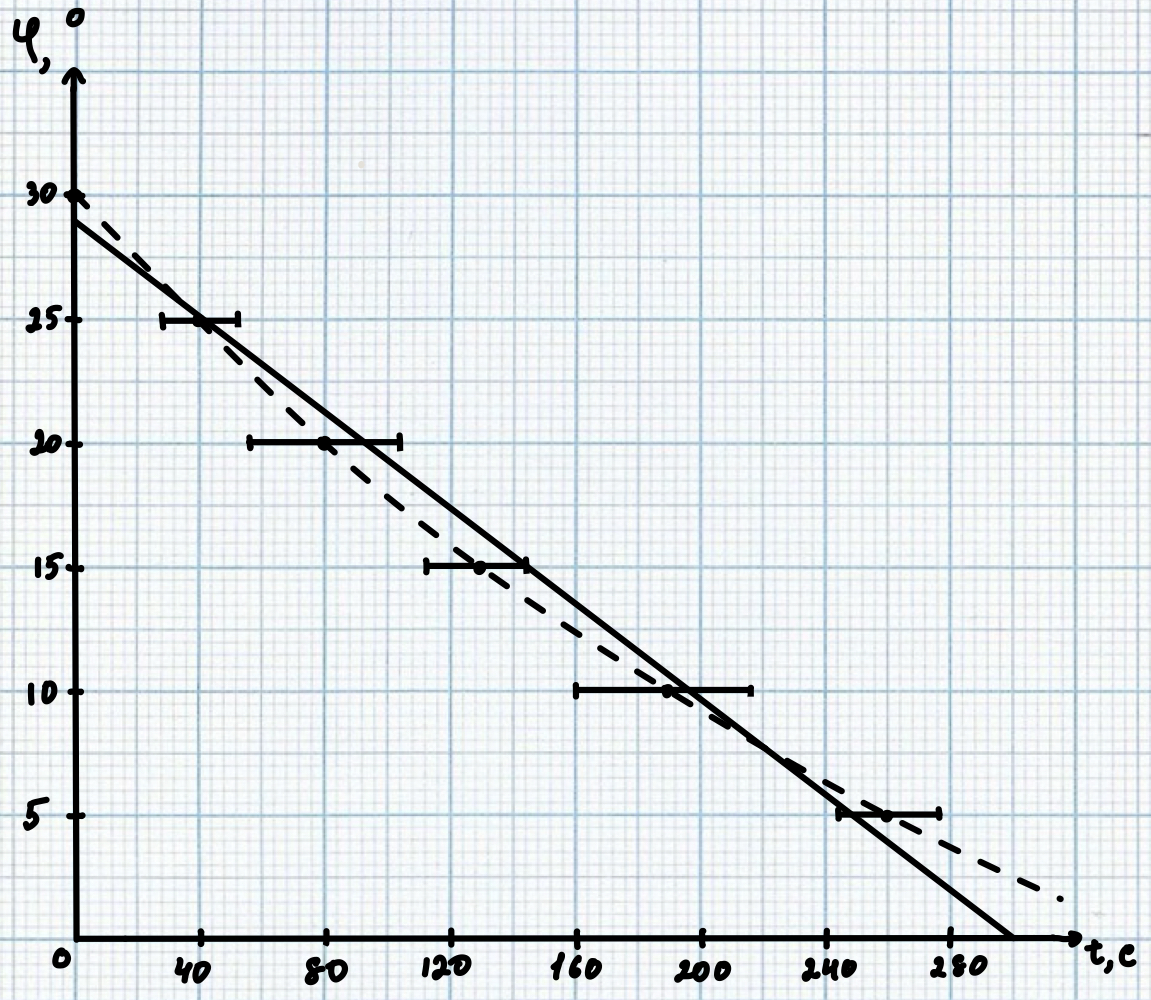
\includegraphics[width=0.7\textwidth]{first.jpeg}\newline
\end{center}
\end{minipage}

\noindent\begin{minipage}{\linewidth}
График зависимости квадрата периода колебаний от момента инерции $T^2=f(I)$, аппроксимирующая прямая и соответствующие экспериментальные точки:

\begin{center}
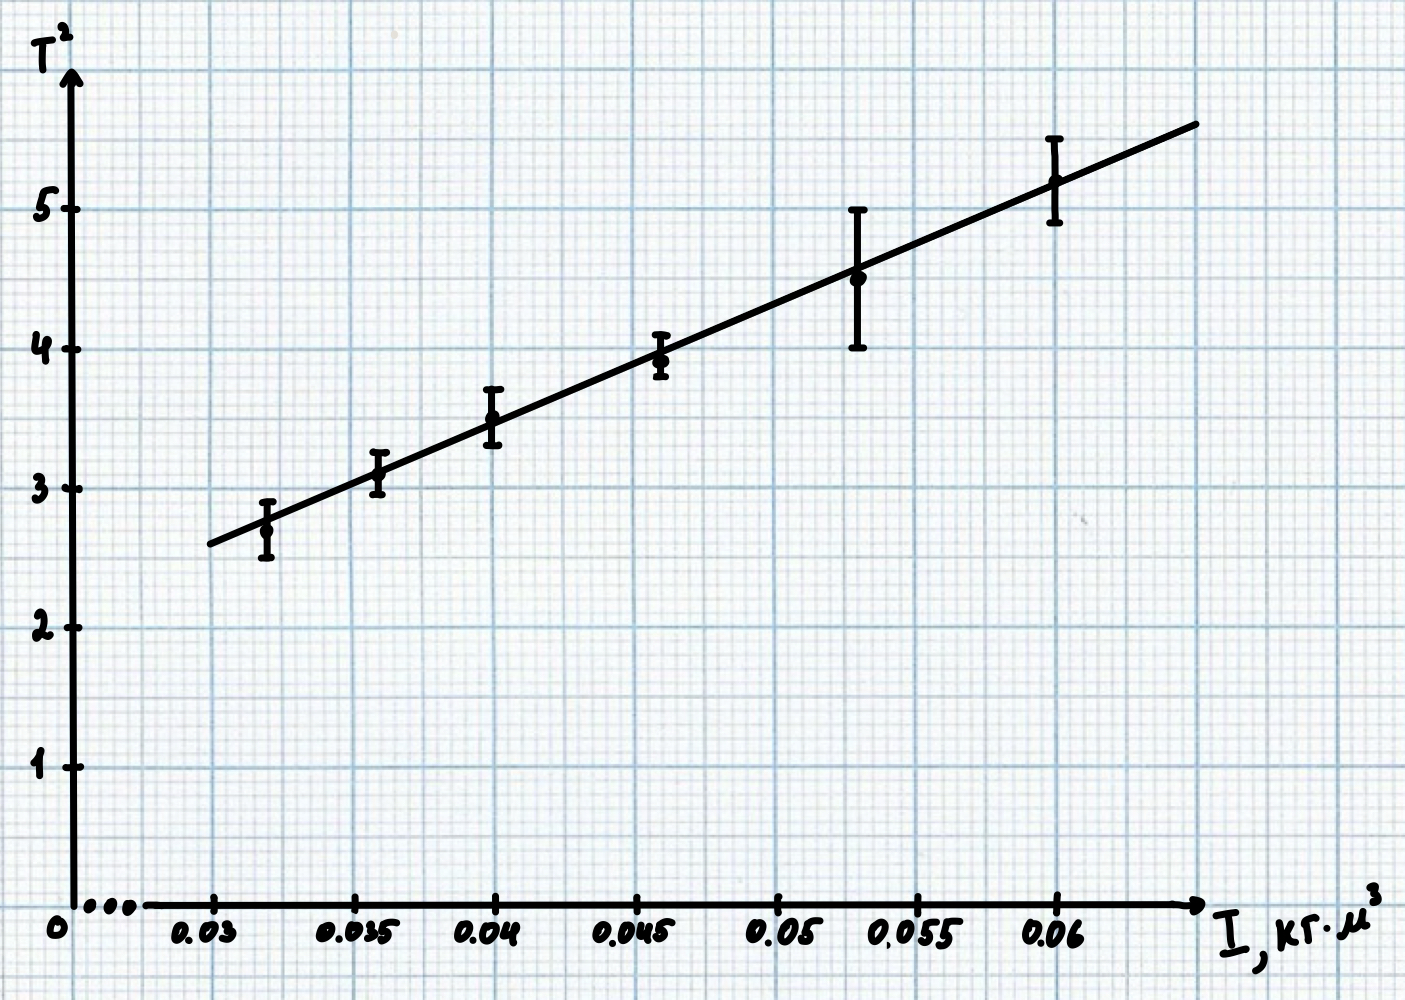
\includegraphics[width=0.7\textwidth]{second.jpeg}\newline
\end{center}
\end{minipage}
\clearpage
% ---------------------------------------------------------------- 12
\sect{12. Окончательные результаты.}

Период колебаний при $\varphi_0=30\gr$:
\begin{itemize}
  \item $T=(1,85\pm0,11)$ с;\quad $\delta_T=6,0\,\%$.
\end{itemize}

Зависимость $\varphi=f(t)$ (преобладает сухое трение):
\begin{itemize}
  \item $\varphi(t)=(28,7\pm1,6)-(0,095\pm0,011)\,t$ (в градусах).
  \item Полуширина зоны застоя $\varphi_\sub{з}=(0,0442\pm0,0057)\gr$;\quad $\delta_{\varphi_\sub{з}}=13\,\%$.
  \item Колебания прекратятся примерно через 169 периодов ($t_\sub{ост}\approx313$ с).
\end{itemize}

Зависимость $T^2=f(I)$:
\begin{itemize}
  \item $T^2=(-0,07\pm0,11)+(87,1\pm2,5)\,I$
  \item $m\ell=(0,0461\pm0,0013)$ кг$\cdot$м;\quad $m\ell_\sub{теор}=(0,0510\pm0,0005)$ кг$\cdot$м;\quad расхождение $9,5\,\%$.
\end{itemize}

Приведённая длина маятника:
\begin{itemize}
  \item Риска 1: $\ell_\sub{пр эксп}=(667\pm40)$ мм;\quad $\ell_\sub{пр теор}=626$ мм;\quad $\delta_\sub{откл}=6,6\,\%$
  \item Риска 2: $\ell_\sub{пр эксп}=(760\pm37)$ мм;\quad $\ell_\sub{пр теор}=697$ мм;\quad $\delta_\sub{откл}=9,0\,\%$
  \item Риска 3: $\ell_\sub{пр эксп}=(863\pm53)$ мм;\quad $\ell_\sub{пр теор}=789$ мм;\quad $\delta_\sub{откл}=9,4\,\%$
  \item Риска 4: $\ell_\sub{пр эксп}=(971\pm27)$ мм;\quad $\ell_\sub{пр теор}=900$ мм;\quad $\delta_\sub{откл}=7,9\,\%$
  \item Риска 5: $\ell_\sub{пр эксп}=(1130\pm110)$ мм;\quad $\ell_\sub{пр теор}=1032$ мм;\quad $\delta_\sub{откл}=9,1\,\%$
  \item Риска 6: $\ell_\sub{пр эксп}=(1291\pm77)$ мм;\quad $\ell_\sub{пр теор}=1184$ мм;\quad $\delta_\sub{откл}=9,1\,\%$
\end{itemize}

Интервальная оценка:
\begin{itemize}
  \item Начальная амплитуда $\varphi_0=30\gr$ попадает в доверительный интервал свободного члена прямой $\varphi(t)$: $27,1$–$30,3\gr$.
  \item Теоретическое $m\ell_\sub{теор}=0,0510$ кг$\cdot$м не попадает в доверительный интервал $m\ell$: $0,0448$–$0,0474$ кг$\cdot$м.
\end{itemize}
% ---------------------------------------------------------------- 13
\sect{13. Выводы и анализ результатов работы.}

Анализ зависимости $\varphi=f(t)$:
\begin{itemize}
  \item Амплитуда уменьшилась с $30\gr$ до $5\gr$ за 261 с; график $\varphi=f(t)$ уменьшается на одну и ту же величину и точки в пределах погрешностей ложатся на прямую, т.е. в затухании преобладает сухое трение в оси подвеса.
  \item Полуширина зоны застоя $\varphi_\sub{з}=(0,0442\pm0,0057)\gr$; маятник остановится примерно через 169 периодов
  ($t_\sub{ост}\approx313$ с).
\end{itemize}

Анализ зависимости $T^2=f(I)$:
\begin{itemize}
  \item При перемещении боковых грузов с 1 на 6 риску момент инерции растёт с 0,0319 до 0,0604 кг$\cdot$м$^2$, а период — с 1,638 до 2,278 с.
  \item Экспериментальные точки $T^2(I)$ в пределах погрешностей ложатся на прямую, а свободный член
  $a=(-0,07\pm0,11)$ с$^2$ совпадает с нулём. Это подтверждает зависимость $T^2\propto I$, т.е. $T=2\pi\sqrt{I/(mg\ell)}$
  (формула (14)): период пропорционален корню из момента инерции.
\end{itemize}

Основной вклад в погрешности вносит не инструментальная погрешность секундомера ($0,01$ с), а случайная
погрешность ручного запуска и остановки секундомера и визуального отсчёта амплитуды. Для повышения точности
следует увеличить число измерений и число отсчитываемых колебаний $N$.

% ---------------------------------------------------------------- 14-16
\sect{14. Дополнительные задания.}

\sect{15. Выполнение дополнительных заданий.}

\sect{16. Замечания преподавателя (исправления, вызванные замечаниями преподавателя, также помещают в этот пункт).}

\vspace{1.5cm}

\begin{tabular}{@{}l@{\ }p{14.5cm}@{}}
Примечание: & 1. Пункты 1-6,8-13 Протокола-отчета обязательны для заполнения.\\
 & 2. Необходимые исправления выполняют непосредственно в протоколе-отчете.\\
 & 3. При ручном построении графиков рекомендуется использовать миллиметровую бумагу.\\
 & 4. Приложения 1 и 2 вкладывают в бланк протокола-отчета.\\
\end{tabular}

\end{document}